\renewcommand\thechapter{\Roman{chapter}}
\chapter{RESULTADOS} \label{ch:resultados} \thispagestyle{fancy}
\renewcommand\thechapter{\arabic{chapter}}
%%%%%%%%%%%%%%%%%%%%%%%%%%%%%%%%%%%%%%%%%%%%%%%%%%%%%%%%%%%%%%%%%%%%%%%%%%%%

En este capítulo se muestra hasta donde se logra llegar, cual es el estado actual del laboratorio virtual. Lo que se muestra a continuacion son resultados parciales del proyecto.\\

Se logra llegar a lo que viene siendo un panel de control el cual controlará un manipulador de 3 GDL, también se observa el modelo en 3D hecho en V-Realm Builder diseñado con piezas sencillas del mismo programa el cual se menciona en el capítulo anterior que las piezas se deben posicionar en un espacio mediante coordenadas para poder alinear las figuras entre si y formar el brazo en este caso.\\

Se muestra en la Figura \ref{matlabescritorio} del lado izquierdo el manipulador en el programa V-Realm Builder, del lado derecho está el panel de control que muestra los botones y los sliders.
El primer slider sirve para mover la parte morada del manipulador, tenemos que realiza giros de -180 a 180, la posición en la que se encuentra es la 0, el segundo slider mueve la parte verde de 0 a 180. el tercer slider mueve lo que viene siendo la posición de la muñeca de igual forma de 0 a 180, por último tenemos la opción del giro de la pinza que viene siendo la herramienta de 0 a 180.\\
Falta crear un enlace mediante código para poder hacer uso del panel con el robot y que se logren captar los movimientos en tiempo real. Se menciona en el capítulo anterior que el archivo GUIDE crea un scrip, dentro de éste es donde se modifican las funciones creadas para poder enlazar el panel y hacer utilidad del mismo para que el usuario interactúe finalmente con el manipulador y sea un paso mas a lo que se quiere llegar, que finalmente son cálculos de cinemáticas.

\begin{figure}{!h}
\centering
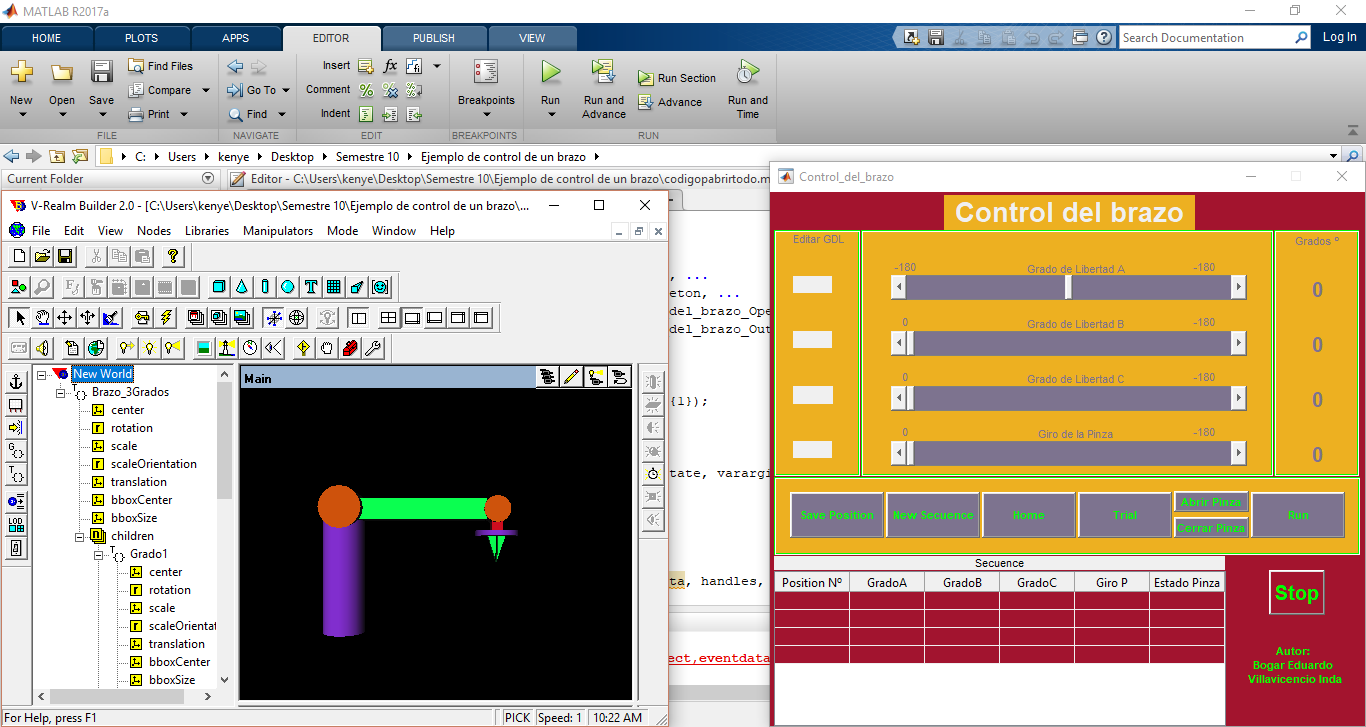
\includegraphics[width=0.9\textwidth, height=0.35\textheight]{./figs/matlabescritorio}\\
\caption{panel de control y robot en 3D.}
\label{matlabescritorio}
\end{figure}